\documentclass{beamer}
\usepackage[utf8]{vietnam}
\usepackage{tikz}
\begin{document}
	\begin{frame}[t,fragile]{Horner scheme (since 1819) - Lược đồ Horner}{$P(x)=(x-a)Q(x)+r$ }
		$P(x)=2x^3-10x^2+17x-15=0$ has a solution $\color{orange}x=3$. 
		\begin{align*}
			P(x)&=2x^3-6x^2-4x^2+12x+5x-15\\
			&=2x^2{\color{orange}(x-3)}-4x{\color{orange}(x-3)}+5{\color{orange}(x-3)}\\
			&={\color{orange}(x-3)}\left(2x^2-4x+5\right)
		\end{align*}
		Horner scheme for $P(x)$ at $\color{orange}x=3$ is as follows. 
		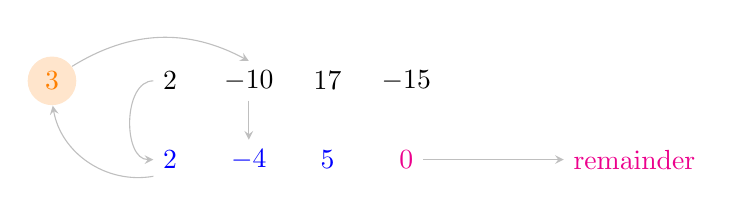
\begin{tikzpicture}[>=stealth]
			\path[nodes={baseline = (2a.base)}] 
			(0,0) node (2a) {$2$}
			++(0:1) node (plus) {$-10$}
			++(0:1) node{$17$}
			++(0:1) node{$-15$}
			(2a)++(0,-1) node[blue] (2b) {$2$};
			\path[nodes={baseline = (2b.base)}] 
			(2b)
			++(0:1) node[blue] (end) {$-4$}
			++(0:1) node[blue]{$5$}
			++(0:1) node[magenta] (R) {$0$}
			;
			\draw[gray!50,->] 
			(2a.180) to[out=180,in=180] (2b.180);
			\draw[gray!50,->] (R)--+(0:2)
			node[right,magenta]{remainder};
			\path (2a) +(180:1.5) node[circle,text=orange,fill=orange!20] (x) {$3$};
			\draw[gray!50,->] (2b.-135) to[bend left=45] (x);
			\draw[gray!50,->] (x) to[bend left] (plus.90);
			\draw[gray!50,->] (plus) to (end);
			%\draw[] (2b.base)--(R.base);
		\end{tikzpicture}
		\vspace{5mm}
		
		Guess:\quad  $2x^3-10x^2+17x+{\color{green}20}=(x-3)(2x^2-4x+5)+{\color{magenta}35}$.
	\end{frame}
\end{document}